\section{Introduction}
% no \IEEEPARstart

\subsection{History}
Blockchain was introduced for the first time about 10 years ago, when Satoshi
Nakamoto, an anonymous Japanese\footnote{Actually, experts thinks that Satoshi
Nakamoto is an alias for a group of people and that no one with that name
really exists.} user in 2008 designed it in order to create a virtual currency,
Bitcoin. Since then, the Blockchain technology has developed to new frontiers,
establishing new ways to interpret money and payments. Not only, it's currently
studied in different fields than the financial one.

\subsection{Blockchain overview}
Blockchain was designed in order to solve the double-spending problem in
online transactions without any third party checking\cite{nakamoto08}. To
achieve this, it rely on a peer-to-peer system, where every user hold a copy of
the whole database.

Every transaction is hashed and stored in a block, and blocks are connected in
a list. These block are generated by the network members, in a process called
`mining'. When users are mining, they contribute generating and validating new
blocks, thanks to the `proof-of-work' puzzles. When a block is generated, a
reward is released from the network, that compensate the users that spent
computational time to generate and validate the transaction block.

Blockchain database differs from other types of databases because it doesn't
allow to modify or delete saved data, but only to add new information.

\subsection{Technical Analysis}

As mentioned above, a Blockchain database is composed of different
parts\cite{sok15}:
\begin{itemize}
 \item Transactions
 \item Blocks concatenated in a list
 \item Peer-to-peer network
\end{itemize}

In this section we will see every component and how its behavior.

\subsubsection{Transactions}
A transaction represents a move of value from a user $A$ to another (let's say
$B$). It contains a list of outputs and an array of inputs\cite{sok15}, and
the sum of the outputs must be less or equal than the sum of the inputs. A
transaction is hashed usually with SHA-256, in order to gain a unique ID.

A transaction change the state of the database, and this change need to be saved
in the database itself. So the database is a list of growing transactions.
In order to validate a transaction, we need to sign it in some way. Thanks to
asymmetric keys the user $A$ can use his public key to sign it.

% To check carefully
So the transaction's ID is processed with $A$ public key, and then the result
is signed with the $A$ private key.

\begin{figure}[H]
 \centering
 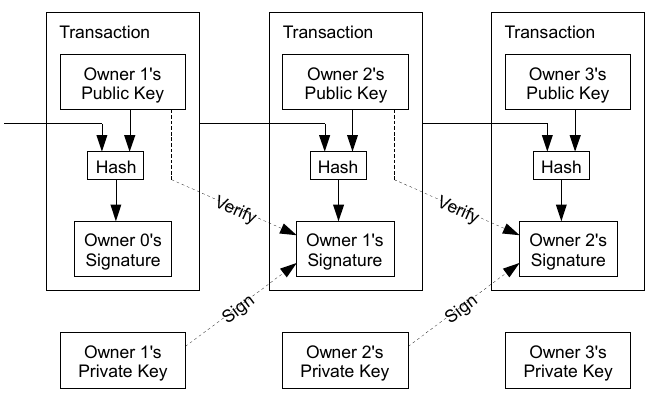
\includegraphics[scale=0.5]{transactions}
 \caption{A transaction scheme (taken from\cite{nakamoto08})}
\end{figure}

Several problems arise from this:
\begin{itemize}
 \item The user $A$ could try to spend two times the same value
 \item No one can guarantee the transaction validity
\end{itemize}
